%%%%%%%%%%%%%%%%%%%%%%%%%%%%%%%%%%%%%%%%%
% Structured General Purpose Assignment
% LaTeX Template
%
% Template Name: Anthony
% The template was named after my friend Anthony.
% Strong inspired by Apache Hadoop and Java (programming language)
%
% Author: Ang LEE
%
% Blog: http://angli.me/
%
% Github: https://github.com/leeang/
%
%%%%%%%%%%%%%%%%%%%%%%%%%%%%%%%%%%%%%%%%%

%----------------------------------------------------------------------------------------
%	CONSTANTS
%----------------------------------------------------------------------------------------

\newcommand{\hmwkTitle}{Report\ \#2 B \& C}				% Assignment title
\newcommand{\hmwkClass}{Signal Processing}				% Course name
\newcommand{\hmwkClassTime}{}							% Workshop time
\newcommand{\hmwkClassInstructor}{}						% Tutor name
\newcommand{\hmwkAuthorName}{Ang LEE}					% Student name

\newcommand{\hmwkGraphicsPath}{img/}					% Graphics path
\newcommand{\hmwkCodePath}{code/}						% Code path

%----------------------------------------------------------------------------------------
%	TEMPLATE
%----------------------------------------------------------------------------------------

\documentclass{article}

\usepackage{fancyhdr}	% Required for custom headers
\usepackage{lastpage}	% Required to determine the last page for the footer
\usepackage{extramarks} % Required for headers and footers
\usepackage{graphicx}	% Required to insert images
\graphicspath{\hmwkGraphicsPath}
\usepackage{lipsum} 	% Used for inserting dummy 'Lorem ipsum' text into the template

\usepackage{float}
\usepackage{epstopdf}	% Required to insert .eps images
\usepackage{amssymb}
\usepackage{amsmath}
\usepackage[hidelinks]{hyperref}

% MATLAB syntax highlighting
\usepackage{color}		% Required to define colors
\definecolor{commentColor}{RGB}{34,139,34}
\definecolor{stringColor}{RGB}{160,32,240}
\usepackage{listings}
\lstset{
	inputpath=\hmwkCodePath,
	language=Matlab,
	basicstyle=\footnotesize\ttfamily,
	keywordstyle=\color{blue},
	stringstyle=\color{stringColor},
	commentstyle=\usefont{T1}{pcr}{m}{n}\color{commentColor},
	breaklines=true,
	showstringspaces=false
}

% Margins
\topmargin=-0.45in
\evensidemargin=0in
\oddsidemargin=0in
\textwidth=6.5in
\textheight=9.0in
\headsep=0.25in

\linespread{1.1}		% Line spacing

% Set up the header and footer
\pagestyle{fancy}
\lhead{\hmwkTitle} % Header Left 
\chead{\hmwkAuthorName} % Header Center
\rhead{\hmwkClass} % Header Right
\lfoot{\url{https://github.com/leeang/Signal-Processing}} % Footer Left
\cfoot{} % Footer Center
\rfoot{Page\ \thepage\ of\ \pageref{LastPage}} % Footer Right
\renewcommand\headrulewidth{0.4pt} % Size of the header rule
\renewcommand\footrulewidth{0.4pt} % Size of the footer rule

\setlength\parindent{0pt} % Removes all indentation from paragraphs

%----------------------------------------------------------------------------------------
%	Problem and Section
%----------------------------------------------------------------------------------------

\newenvironment{homeworkProblem}[1]{
	\section*{#1}
	}{
}
\newenvironment{homeworkSection}[1]{
	\subsection*{#1}
	}{
}
\newcommand{\problemAnswer}[1]{
	\noindent\framebox[\columnwidth][c]{
		\begin{minipage}{0.98\columnwidth}
			#1
		\end{minipage}
	}
}

%----------------------------------------------------------------------------------------
%	Document
%----------------------------------------------------------------------------------------

\begin{document}

\newpage

%----------------------------------------------------------------------------------------
%	PROBLEM B a
%----------------------------------------------------------------------------------------

\begin{homeworkProblem}{B a)}

\begin{homeworkSection}{(\romannumeral1)}

From part A question 2, the impulse response of 
\begin{equation}
H_1(z)=1+\alpha z^{-1}=\alpha^0 z^{-0}+\alpha z^{-1}
\end{equation}
can be shown as  
\begin{equation}
h_1[n]=\sum_{i=0}^{1}\alpha^i\delta[n-i]=\alpha^0\delta[n]+\alpha\delta[n-1]
\end{equation}
Now the filter becomes
\begin{equation}
H_1(z^D) = 1 + \alpha z^{-D}=\alpha^0z^{-0D}+\alpha z^{-D}
\end{equation}
Using time shift property, the corresponding impulse response is 
\begin{equation}
h'_1[n]=\alpha^0\delta[n]+\alpha\delta[n-D]=\delta[n]+\alpha\delta[n-D]
\end{equation}
If we have an input signal $x[n]$ pass through the filter $H(z^D)$, the output $y[n]$ is 
\begin{equation}
y[n]=x[n]+\alpha x[n-D]
\end{equation} 

It can be clearly seen that output signal $y[n]$ is the superposition of the original signal: $x[n]$ and the delayed and attenuated signal: $\alpha x[n-D]$, i.e. ``echo''.

\begin{figure}[H]
\centering
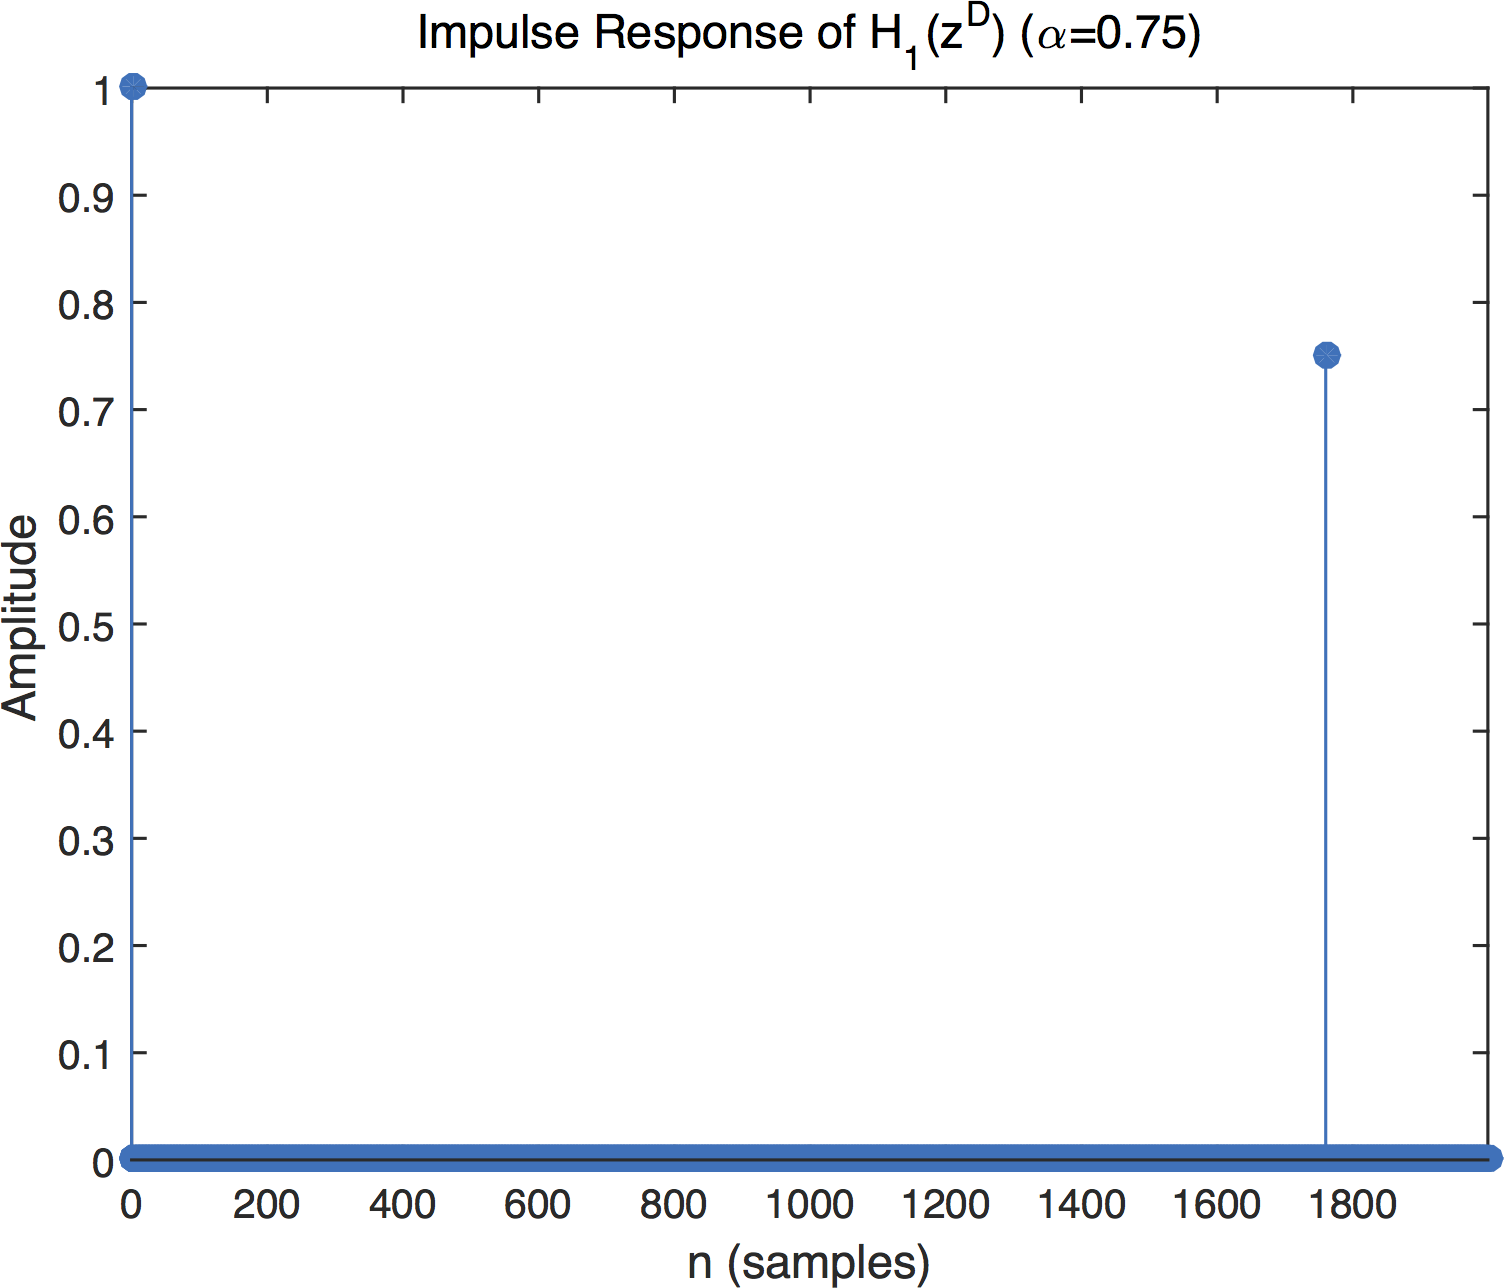
\includegraphics[width=5in]{Ba1}
\caption{Impulse Response $H_1(z^D)$ ($\alpha=0.75$)}
\label{Ba2}
\end{figure}

\end{homeworkSection}

\begin{homeworkSection}{(\romannumeral2)}

Here we set the sampling rate $F_s=8\text{ kHz}$.

\begin{align*}
y[n] &= x[n] + \alpha x[n-D]\\
y(t) &= x(t) + \alpha x(t-\frac{D}{F_s})
\end{align*}

$\frac{D}{F_s}=\text{220 ms} \longrightarrow D = 220 \text{ ms} \times 8\text{ kHz} = 1760 \text{ samples}$\\

$\alpha$ determines the amplification of the original signal. Due to $0< \alpha <1$, the echo is essentially attenuated. For instance, when $\alpha=0.1$, the echo amplitude is only 10\% of the magnitude of the original signal.\\

Larger $D$ implies more delay (samples), in other words, longer time delay(ms).

\end{homeworkSection}

%--------------------------------------------

\begin{homeworkSection}{(\romannumeral3)}
The c code can be seen in Appendix. 
\end{homeworkSection}

%--------------------------------------------

\begin{homeworkSection}{(\romannumeral4)}
We can hear a sound followed by its echoes every time we play it.
\end{homeworkSection}

%--------------------------------------------

\end{homeworkProblem}

%----------------------------------------------------------------------------------------
%	PROBLEM B b
%----------------------------------------------------------------------------------------

\begin{homeworkProblem}{B b)}

\begin{homeworkSection}{(\romannumeral1)}

The frequency response of filter $H_2(z^D)$ is 
\begin{align*}
H_2(e^{j\omega D}) &= \frac{1}{1 + \alpha e^{-j\omega D}}\\
&= \sum_{n=0}^{\infty} (-\alpha)^n e^{-jnD\omega}
\end{align*}
Referring to the conclusion in part A, the impulse response of filter $H_2(z^D)$ is
\begin{equation}
h_2[k]=\sum_{k=0}^{\infty}(-\alpha)^k\delta[n-kD]
\end{equation}

\begin{equation}\label{B2i1}
h[n] =
\begin{cases} (-\alpha)^n & n=kD, k \in \mathbb{Z}_0^{+}\\ 0 & \text{otherwise}\\ \end{cases}
\end{equation}

Response to an arbitrary sequence $\{x[n]\}$ is shown below
\begin{align*}
x[n] &= \sum_{k=-\infty}^{\infty} x[k] \delta[n-k]\\
y[n] &= \sum_{k=-\infty}^{\infty} x[k] h[n-k]\\
&= \sum_{k=-\infty}^{\infty} h[k] x[n-k]\\
&= \sum_{k=0}^{\infty} (-\alpha)^k x[n-kD]\ \ (|\alpha| < 1)
\end{align*}

It can be clearly seen that output signal $y[n]$ is the superposition of the original signal: $x[n]$ and an infinite sequence of delayed and attenuated signals: $(-\alpha)^k x[n-kD]$. Hence, multiple echoes are generated.

\begin{figure}[H]
\centering
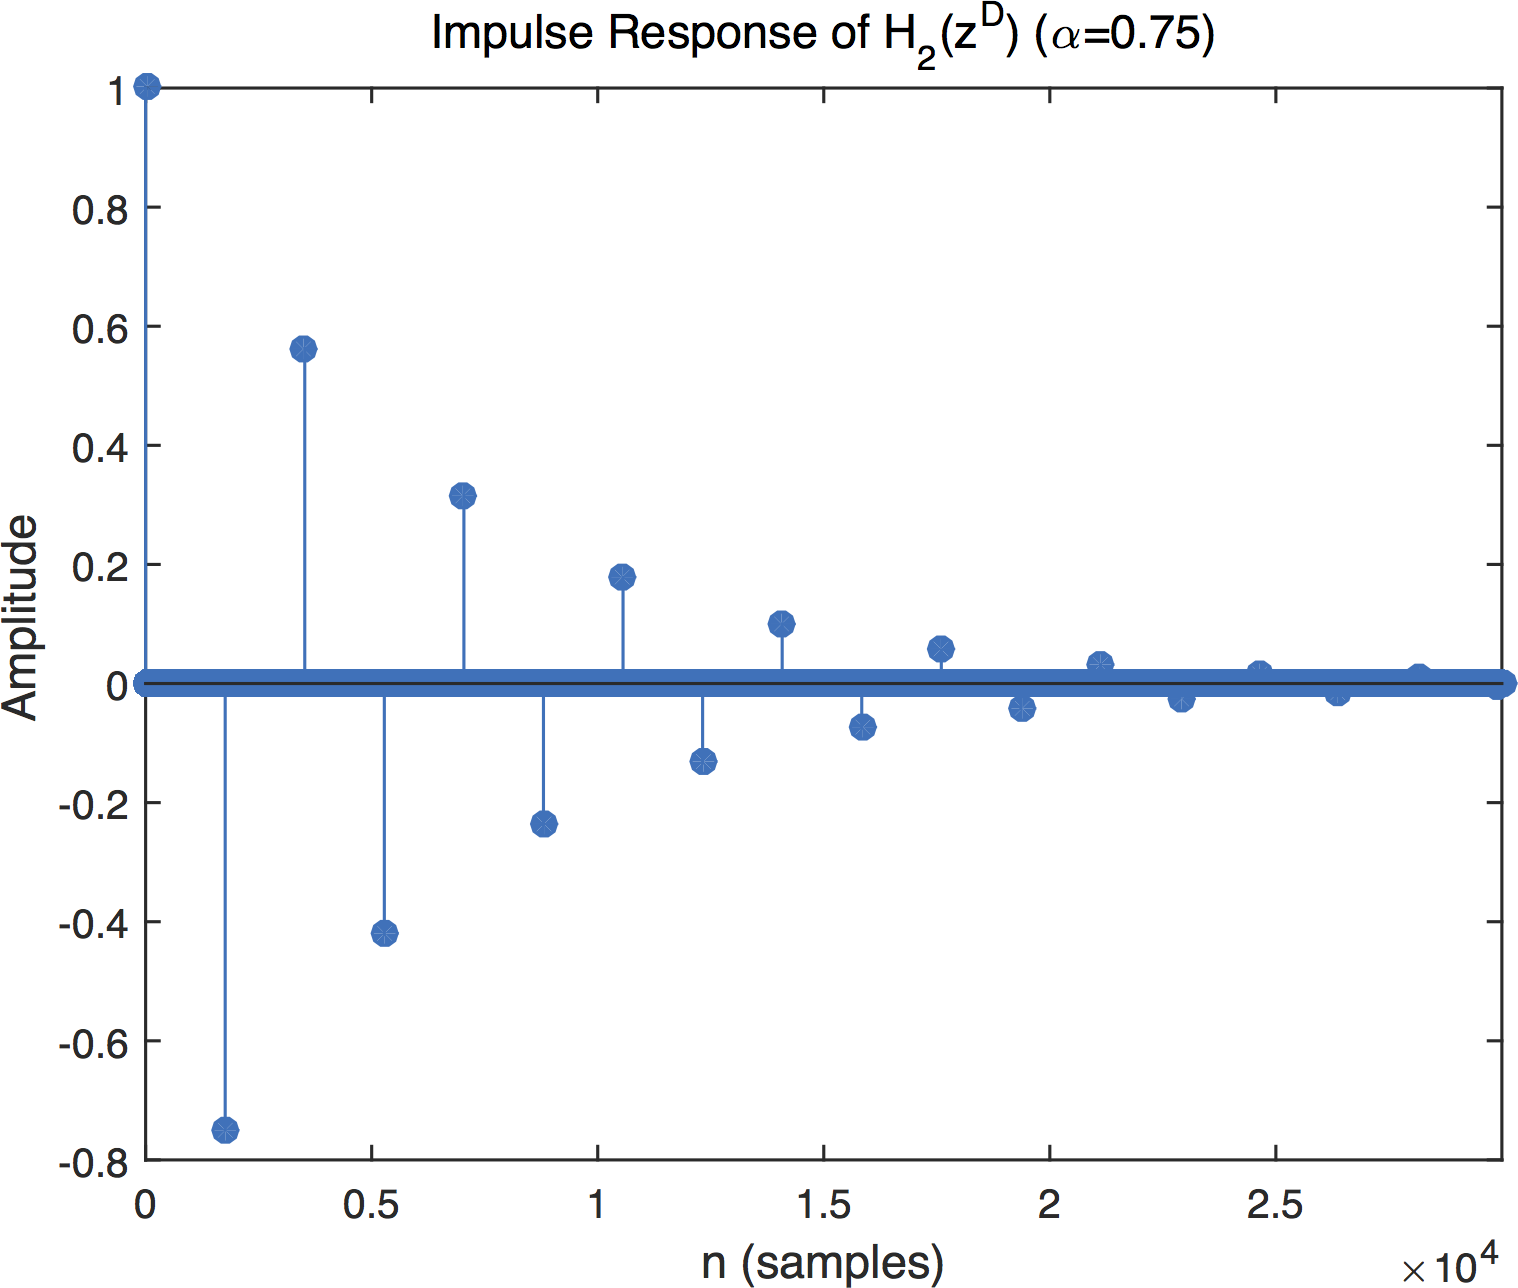
\includegraphics[width=5in]{Bb1}
\caption{Impulse Response $H_2(z^D)$ ($\alpha=0.75$)}
\label{Bb1}
\end{figure}

\end{homeworkSection}

%--------------------------------------------

\begin{homeworkSection}{(\romannumeral2)}

\begin{align*}
y[n] &= x[n] + (-\alpha) x[n-D] + (-\alpha)^2 x[n-2D] + (-\alpha)^3 x[n-3D] + \cdots\\
y(t) &= x(t) + (-\alpha) x(t-\frac{D}{F_s}) + (-\alpha)^2 x(t-\frac{2D}{F_s}) + (-\alpha)^3 x(t-\frac{3D}{F_s}) + \cdots
\end{align*}

$\frac{D}{F_s}=\text{220 ms} \longrightarrow D = 220 \text{ ms} \times 8\text{ kHz} = 1760 \text{ samples}$\\

More echoes and more obvious delays can be heard from the signal generated in b) (ii). The signal generated in b) (ii) sounds louder.

\end{homeworkSection}

%--------------------------------------------

\begin{homeworkSection}{(\romannumeral3)}

\begin{align*}
\sum_{k=0}^{\infty} h_1^2[k] &= \sum_{k=0}^{\infty} h_2^2[k]\\
1^2 + \alpha_1^2 &= 1^2 + (-\alpha_2)^2 + (\alpha_2^2)^2 + (-\alpha_2^3)^2 + \cdots\\
1 + \alpha_1^2 &= \frac{1}{1 - \alpha_2^2}\\
\alpha_2 &= \sqrt{1 - \frac{1}{1 + \alpha_1^2}}\\
\alpha_2 &= 0.6
\end{align*}

\begin{figure}[H]
\centering
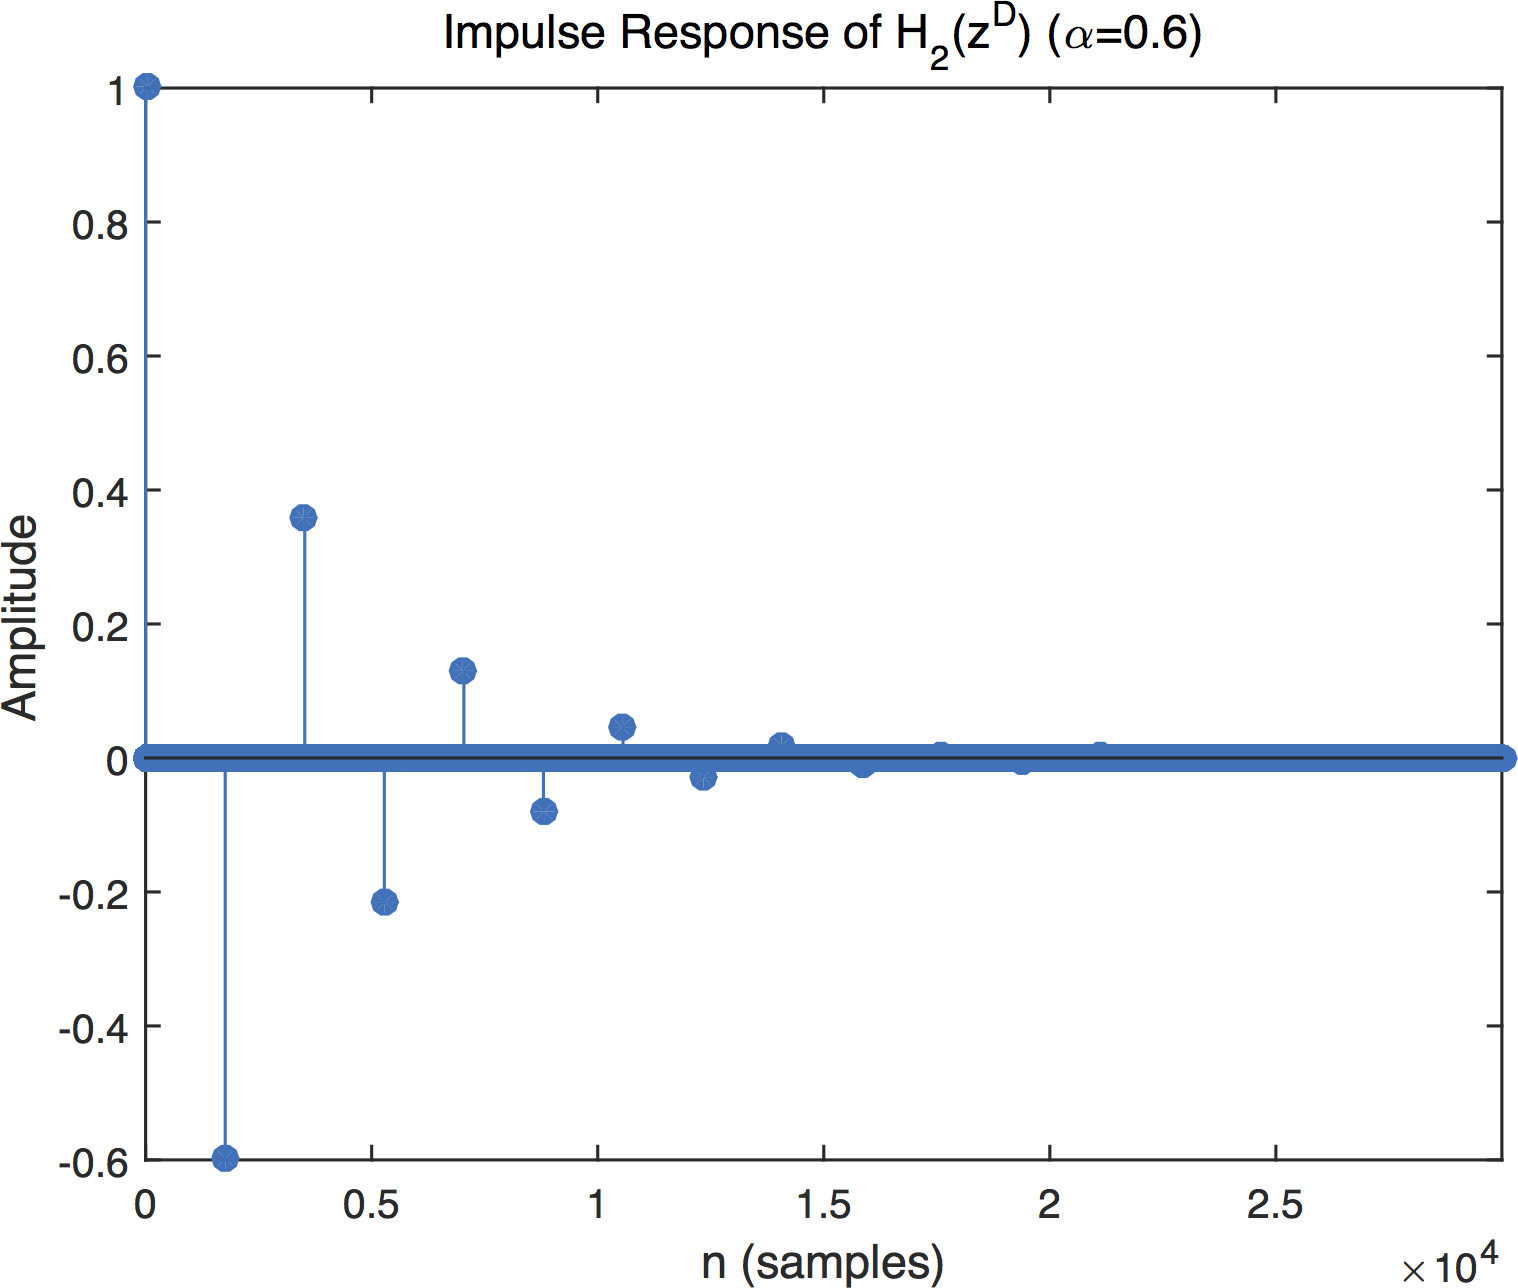
\includegraphics[width=5in]{Bb3}
\caption{Impulse Response $H_2(z^D)$ ($\alpha=0.6$)}
\label{Bb3}
\end{figure}

The signal generated in b) (ii) is slightly louder, especially at the beginning of the audio. As is shown in Figure.\ref{Bb3}, the impulse response of $H_2(z^D)$ consists of infinite impulses, in a relative short time (4 seconds comparing with 220ms delay), only a part of them will present. However, the calculated power of these two signals are the same when $\alpha_2=0.6$ and in infinitely long time.

\end{homeworkSection}

%--------------------------------------------

\begin{homeworkSection}{(\romannumeral4)}

\begin{figure}[H]
\centering
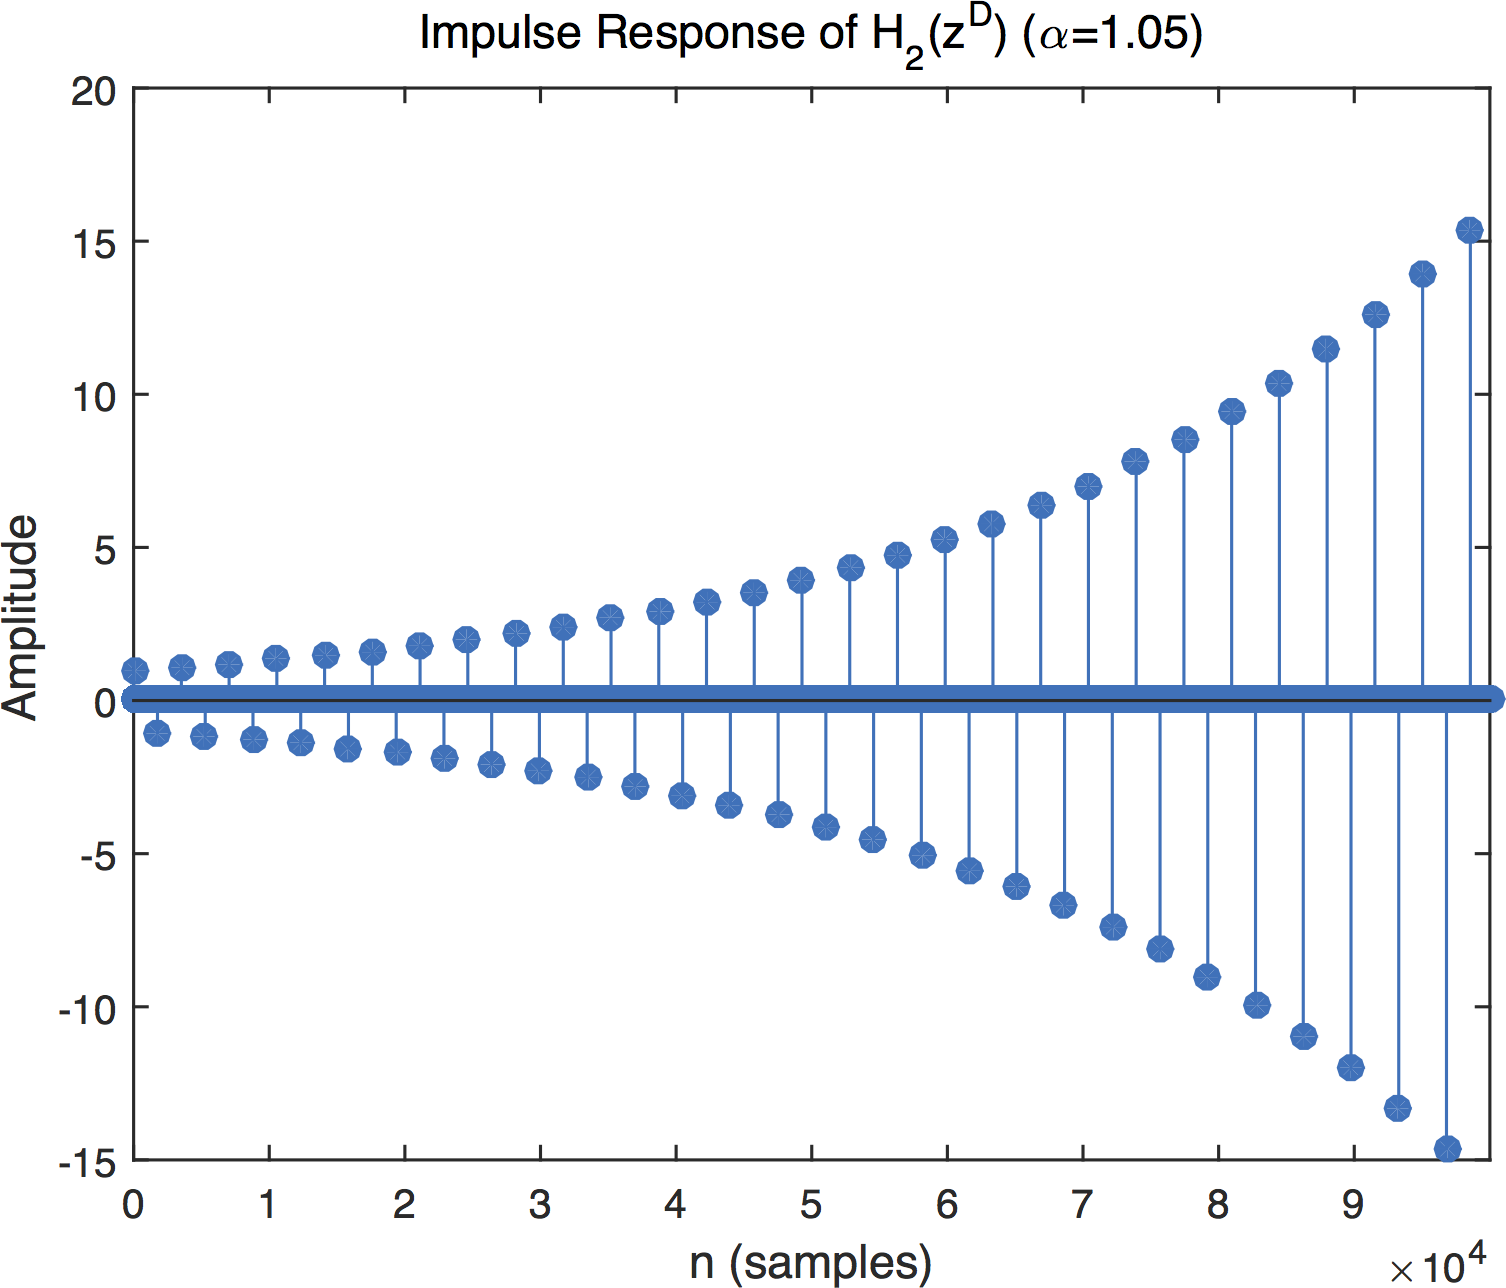
\includegraphics[width=5in]{Bb4}
\caption{Impulse Response $H_2(z^D)$ ($\alpha=1.05$)}
\label{Bb4}
\end{figure}

Echoes crescendo, even louder than the input signal. As $\alpha = 1.05 > 1$, the pole is located outside the unit circle, hence the filter is \textbf{unstable}. As is shown in Figure.\ref{Bb4}, the impulse response diverges.

\end{homeworkSection}

%--------------------------------------------

\begin{homeworkSection}{(\romannumeral5)}

\subsubsection*{Time domain representation}
\begin{align*}
y[n] &= x[n] + (-\alpha) x[n-D] + (-\alpha)^2 x[n-2D] + (-\alpha)^3 x[n-3D] + \cdots\\
y[n-D] &= x[n-D] + (-\alpha) x[n-2D] + (-\alpha)^2 x[n-3D] + (-\alpha)^3 x[n-4D] + \cdots\\
y[n] &= x[n] - \alpha y[n-D]
\end{align*}

The output sound has multiple echoes comparing with the first filter.
\end{homeworkSection}

%--------------------------------------------

\end{homeworkProblem}

%----------------------------------------------------------------------------------------
%	PROBLEM B c
%----------------------------------------------------------------------------------------

\begin{homeworkProblem}{B c)}

\begin{homeworkSection}{(\romannumeral1)}

\begin{figure}[H]
\centering
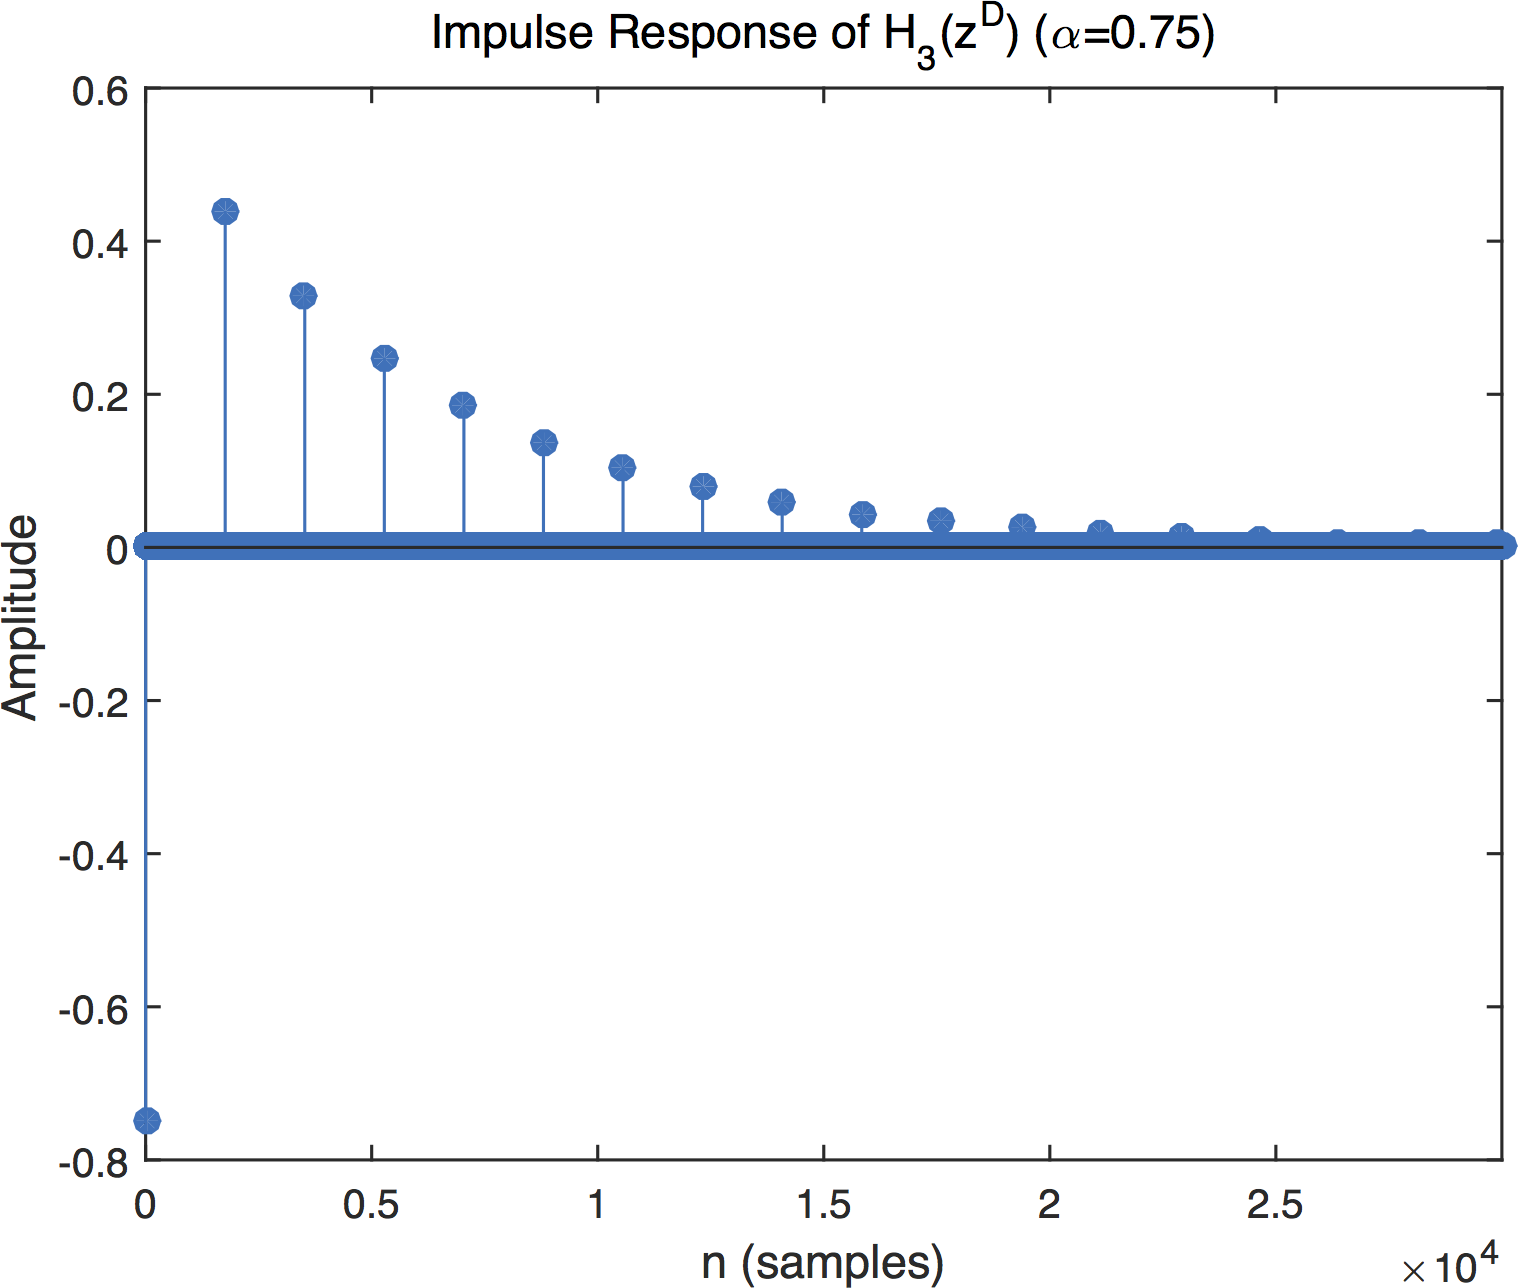
\includegraphics[width=5in]{Bc1}
\caption{Impulse Response $H_3(z^D)$ ($\alpha=0.75$)}
\label{Bc1}
\end{figure}

It can be clearly seen that output signal $y[n]$ is the superposition of the original signal: $x[n]$ and an infinite sequence of delayed and attenuated signals. Hence, $H_3(z^D)$ can be used as an echo filter.

The magnitude response of $H_3(z^D)$ is frequency-invariant, i.e. $|H_3(e^{j\omega})|=1$.\\

By comparing Figure.\ref{Bb1} and Figure.\ref{Bc1}, it can be concluded that the magnitude of impulses(except the first negative impulse) decay much slower in $H_3(z^D)$. In other words, the echo density is higher than the counterparts generated by $H_1(z^D)$ and $H_2(z^D)$. Therefore, $H_3(z^D)$ gives less coloration of the sound.

\end{homeworkSection}

%--------------------------------------------

\begin{homeworkSection}{(\romannumeral2)}

$\frac{D}{F_s}=\text{220 ms} \longrightarrow D = 220 \text{ ms} \times 8\text{ kHz} = 1760 \text{ samples}$\\

This echo generator sounds more natural than the first two and of less coloration. But we still cannot get a smooth sounding reverberation due to obvious separated echoes.

\end{homeworkSection}

%--------------------------------------------

\begin{homeworkSection}{(\romannumeral3)}

\subsubsection*{Time domain representation}
\begin{align*}
H_3(z^D) &= \frac{z^{-D}-\alpha}{1 - \alpha z^{-D}}\\
Y(z) &:= H_3(z^D) X(z)\\
Y(z) - \alpha z^{-D} Y(z) &= z^{-D} X(z) - \alpha X(z)\\
Y(z) &= z^{-D} X(z) - \alpha X(z) + \alpha z^{-D} Y(z)\\
y[n] &= x[n-D] - \alpha x[n] + \alpha y[n-D]
\end{align*}

\end{homeworkSection}

%--------------------------------------------

\end{homeworkProblem}

%----------------------------------------------------------------------------------------
%	PROBLEM B d
%----------------------------------------------------------------------------------------

\begin{homeworkProblem}{B d)}

\begin{homeworkSection}{(\romannumeral1)}

\begin{figure}[H]
\begin{minipage}[t]{0.5\linewidth}
\centering
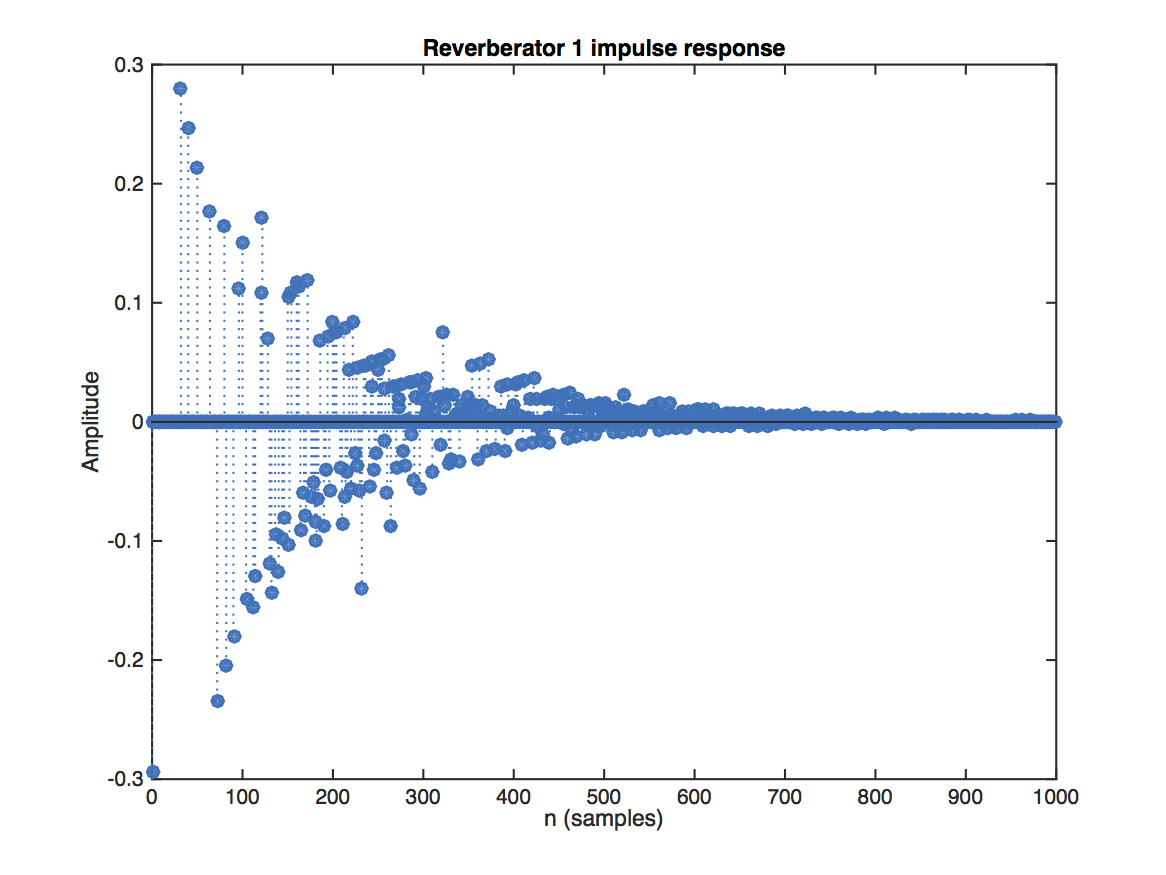
\includegraphics[width=3.3in]{Bd1-1}
\caption{Reverberator 1 impulse response}
\label{Bd1-1}
\end{minipage}
\begin{minipage}[t]{0.5\linewidth}
\centering
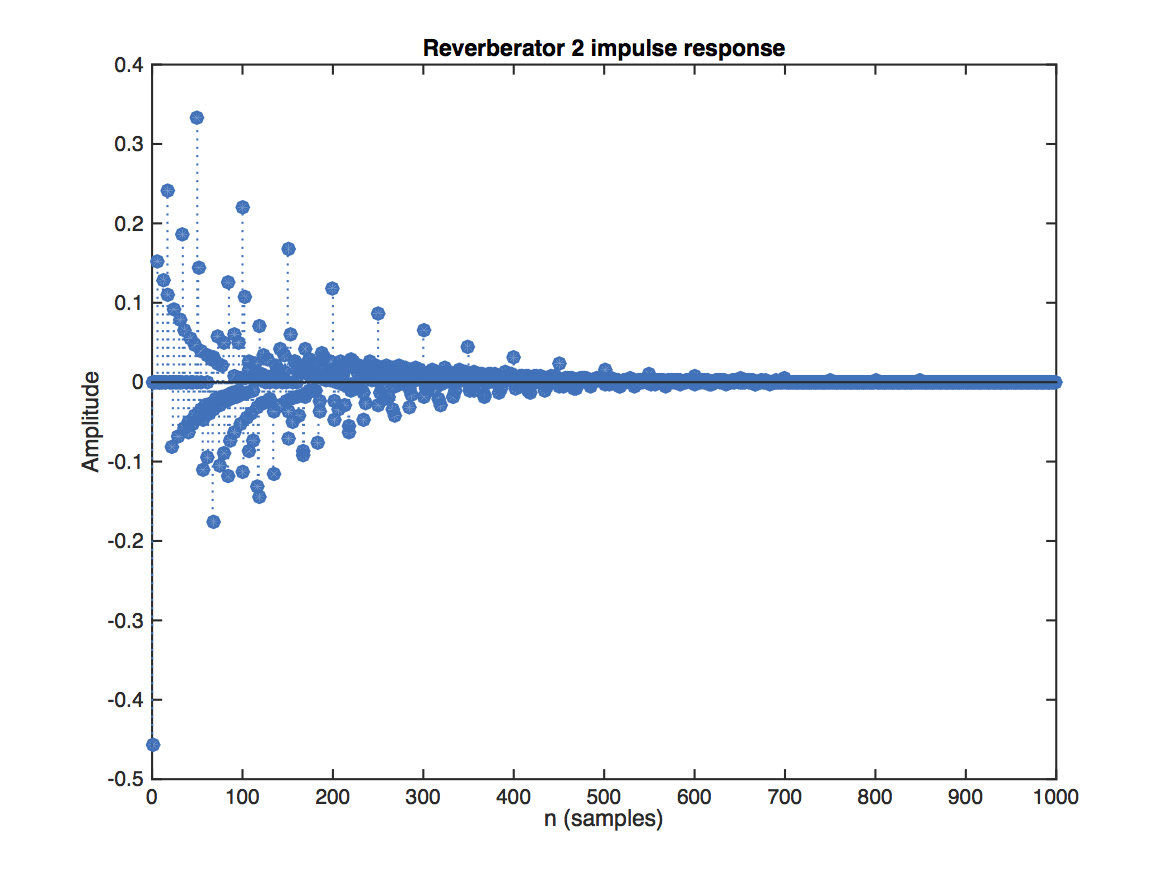
\includegraphics[width=3.3in]{Bd1-2}
\caption{Reverberator 2 impulse response}
\label{Bd1-2}
\end{minipage}
\end{figure}

Reverberator 2 is better. The impulse density is more intensive so that adjacent echoes cannot be differentiated.

\end{homeworkSection}

%--------------------------------------------

\begin{homeworkSection}{(\romannumeral2)}

If $D_{1,2,3}$ are rounded to nearest prime numbers, their echoes will be $nD_{1,2,3}$ and the overlap probability among $nD_1$, $nD_2$ and $nD_3$ is much less than non-prime $D_{1,2,3}$. In other words, the impulse response is much more dense than before.

\end{homeworkSection}

%--------------------------------------------

\begin{homeworkSection}{(\romannumeral3)}

\begin{align*}
D_1 &= 50\text{ ms} \times 8\text{ kHz} = 400 \approx 401\\
D_2 &= 40\text{ ms} \times 8\text{ kHz} = 320 \approx 317\\
D_3 &= 32\text{ ms} \times 8\text{ kHz} = 256 \approx 257
\end{align*}

\begin{figure}[H]
\centering
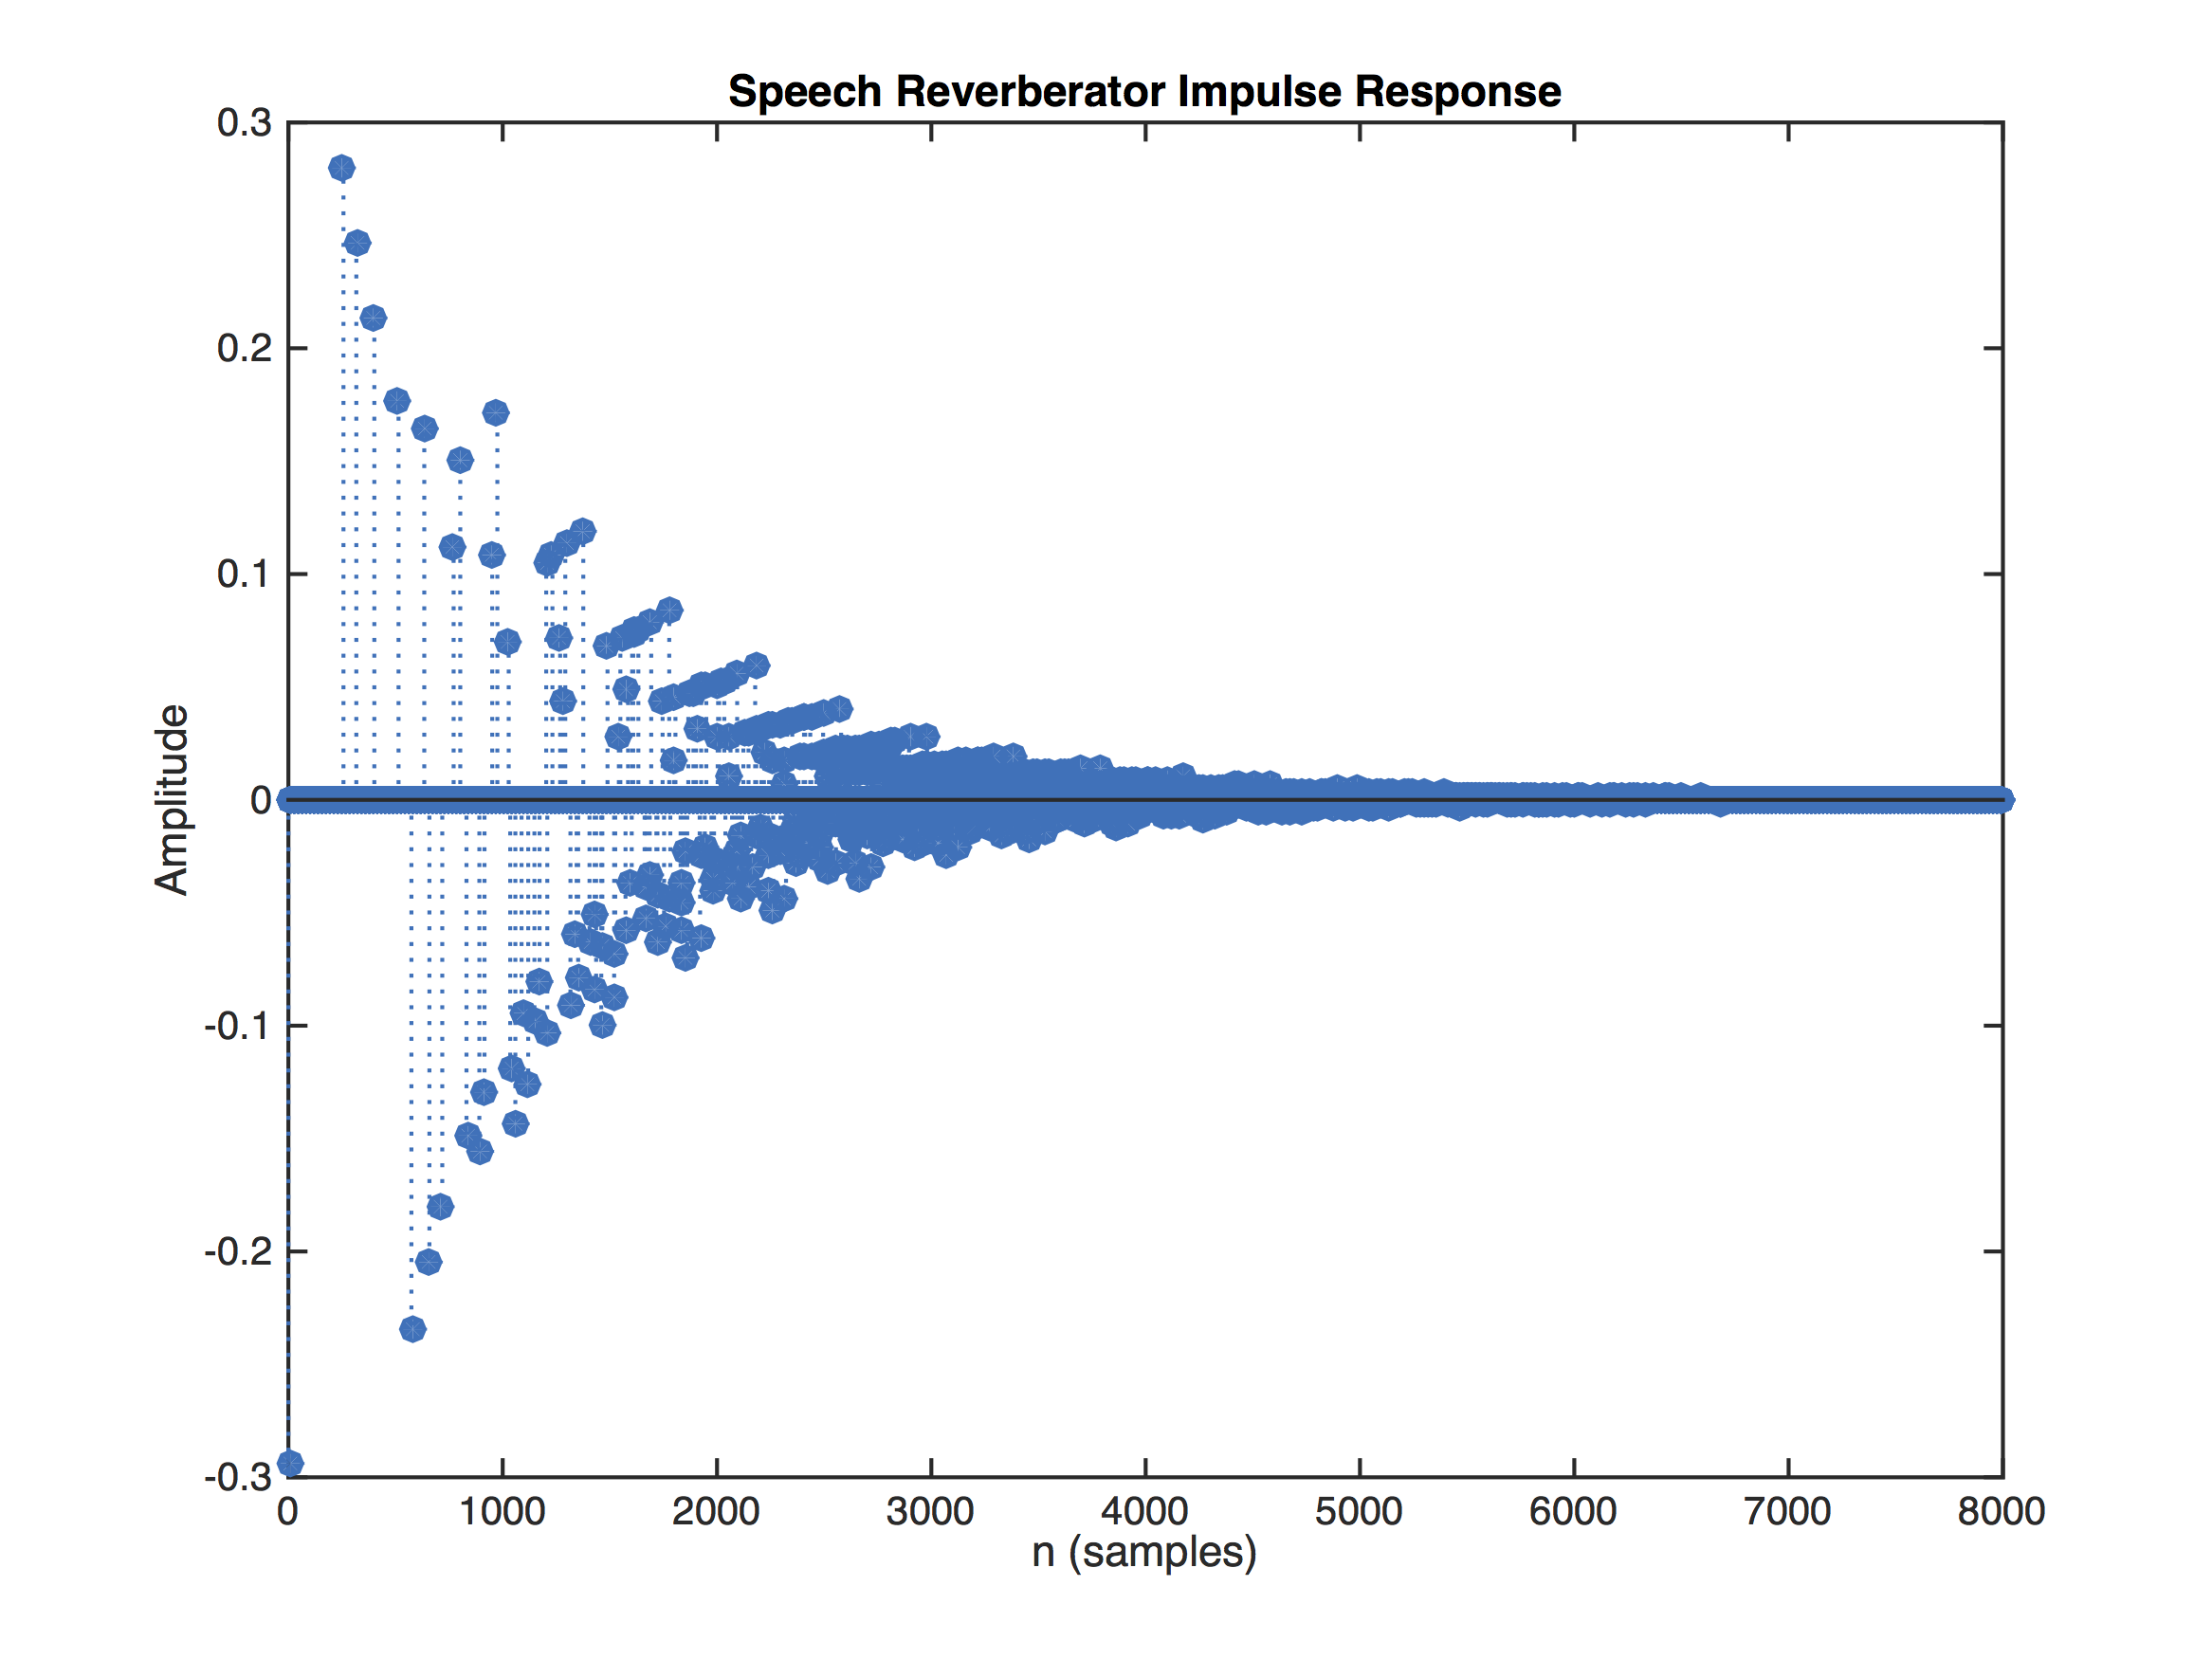
\includegraphics[width=5in]{Bd3}
\caption{Impulse response}
\label{Bd3}
\end{figure}

Comparing Figure.\ref{Bd1-1} and Figure.\ref{Bd3}, the impulse density increases and the sound is more natural.

\end{homeworkSection}

%--------------------------------------------

\end{homeworkProblem}

%----------------------------------------------------------------------------------------
%	PROBLEM C c
%----------------------------------------------------------------------------------------

\begin{homeworkProblem}{C c)}

%--------------------------------------------

\begin{homeworkSection}{AddSinus()}

$F = 550$ Hz\\

\problemAnswer{
\lstinputlisting[language=c]{AddSinus.c}
}

\end{homeworkSection}

%--------------------------------------------

\begin{homeworkSection}{FilterCoeff()}

\begin{equation}\label{Cc1}
\omega_0 = \frac{2\pi \times 550 \text{ Hz}}{24 \times 10^3 \text{ sample/s}} = 0.143990 \text{ rad/sample}
\end{equation}

\begin{equation}\label{Cc2}
H_{BS}(z) = \frac{1+\alpha}{2} \frac{1-2\beta z^{-1} + z^{-2}}{1 - \beta (1+\alpha) z^{-1} + \alpha z^{-2}}
\end{equation}
where $\beta = \cos(\omega_0) = \textbf{0.989651}$.\\

Poles at $r e^{\pm j\phi}$, a stable system requires $r=\sqrt{\alpha}<1$, i.e. $0<\alpha<1$.

\begin{equation}\label{Cc3}
B_w = \cos^{-1}(\frac{2\alpha}{1+\alpha^2})\\
\end{equation}

Given $0<\alpha<1$
\begin{equation}\label{Cc4}
\alpha = \frac{1}{\cos(B_w)} - \sqrt{\frac{1}{(\cos(B_w))^2}-1}
\end{equation}

\problemAnswer{
\lstinputlisting[language=c]{FilterCoeff.c}
}

When $B_w = 0.1\pi$, from Eq. \ref{Cc4}
\begin{equation}
\alpha = 0.726543
\end{equation}

When $B_w = 0.01\pi$, from Eq. \ref{Cc4}
\begin{equation}
\alpha = 0.969067
\end{equation}

When $B_w = 0.0025\pi$, from Eq. \ref{Cc4}
\begin{equation}
\alpha = 0.992177
\end{equation}

\end{homeworkSection}

%--------------------------------------------

\begin{homeworkSection}{Time domain representation}

\begin{align*}
H_{BS}(z) &= \frac{1+\alpha}{2} \frac{1-2\beta z^{-1} + z^{-2}}{1 - \beta (1+\alpha) z^{-1} + \alpha z^{-2}}\\
Y(z) &:= H_{BS}(z) X(z)\\
(1 - \beta (1+\alpha) z^{-1} + \alpha z^{-2}) Y(z) &= \frac{1+\alpha}{2} (1 - 2 \beta z^{-1} + z^{-2}) X(z)\\
y[n] - \beta (1+\alpha) y[n-1] + \alpha y[n-2] &= \frac{1+\alpha}{2} (x[n] - 2 \beta x[n-1] + x[n-2])
\end{align*}

\begin{align*}
y[n] &= \frac{1+\alpha}{2} (x[n] - 2 \beta x[n-1] + x[n-2]) + \beta (1+\alpha) y[n-1] - \alpha y[n-2]\\
&= b_0 x[n] + b_1 x[n-1] + b_2 x[n-2] - a_1 y[n-1] - a_2 y[n-2]
\end{align*}
\begin{align*}
b_0 &= \frac{1+\alpha}{2}\\
b_1 &= 2 \beta \cdot \frac{1+\alpha}{2}\\
b_2 &= \frac{1+\alpha}{2}\\
a_1 &= - \beta (1+\alpha)\\
a_2 &= \alpha
\end{align*}

\end{homeworkSection}

%--------------------------------------------

\end{homeworkProblem}

%----------------------------------------------------------------------------------------
%	PROBLEM C d
%----------------------------------------------------------------------------------------

\begin{homeworkProblem}{C d)}

%--------------------------------------------

When smaller bandwidths ($0.1\pi \to 0.01\pi \to 0.0025\pi$) are adopted, the filtered signal sounds clearer.

%--------------------------------------------

\end{homeworkProblem}

%----------------------------------------------------------------------------------------
%	Appendix
%----------------------------------------------------------------------------------------

\newpage
\begin{homeworkProblem}{Appendix}

\begin{homeworkSection}{SPWS2-echo/\_LabTasks.c}
	\lstinputlisting[language=c]{echo.c}
\end{homeworkSection}

\newpage
\begin{homeworkSection}{SPWS2-notch/\_LabTasks.c}
	\lstinputlisting[language=c]{notch.c}
\end{homeworkSection}

\newpage
\begin{homeworkSection}{B a) (\romannumeral2)}
	\lstinputlisting{Ba2.m}
\end{homeworkSection}

\begin{homeworkSection}{B b) (\romannumeral2)}
	\lstinputlisting{Bb2.m}
\end{homeworkSection}

\begin{homeworkSection}{B b) (\romannumeral3)}
	\lstinputlisting{Bb3.m}
\end{homeworkSection}

\begin{homeworkSection}{B b) (\romannumeral4)}
	\lstinputlisting{Bb4.m}
\end{homeworkSection}

\begin{homeworkSection}{B c) (\romannumeral2)}
	\lstinputlisting{Bc2.m}
\end{homeworkSection}

\begin{homeworkSection}{B d) MATLAB function}
	\lstinputlisting{Bd_function.m}
\end{homeworkSection}

\begin{homeworkSection}{B d) (\romannumeral1)}
	\lstinputlisting{Bd1.m}
\end{homeworkSection}

\begin{homeworkSection}{B d) (\romannumeral3)}
	\lstinputlisting{Bd3.m}
\end{homeworkSection}

\end{homeworkProblem}

%----------------------------------------------------------------------------------------

\end{document}
